% Provenance (never printed): see sources/outline_sources.md (Year 1: optical
% mineralogy with the polarising microscope; Michel-Levy chart). Interference
% colours in figdata/bachelor-1/michel_levy.py from the CIE 1931 colour-matching
% functions and illuminant D65 (data/derived/bachelor-1-cie*.csv); exercise and
% problem values in the Book 3 scratch calculator calc/ch08.py.
\chapter{प्रकाशिकी खनिजविज्ञान}\label{ch:b1:optical-mineralogy}

\omterm{def:b1:field-lab-methods-1:microscope}{आड़े ध्रुवकों} के बीच एक गैब्रो की \omterm{def:b1:field-lab-methods-1:thin-section}{पतली काट} रंगीन काँच की खिड़की की तरह चमकती है। लंबे धूसर और सफ़ेद पत्थर, बारकोड
की तरह धारीदार, क्षेत्र को पार करते हैं; उनके बीच कण नीले, पीले और मैजेंटा रंग में दमकते हैं; कुछ कोण चाहे जो
हो, काले रहते हैं। इनमें से हर प्रभाव का एक परिकलित हो सकने वाला कारण है, और हर एक बताता है कि वहाँ कौन-सा
\omterm{def:b1:rock-forming-minerals:mineral}{खनिज} है। यह अध्याय बताता है कि प्रकाश एक क्रिस्टल से कैसे गुज़रता है, \omterm{def:b1:field-lab-methods-1:microscope}{आड़े ध्रुवकों} के बीच एक \omterm{def:b1:rock-forming-minerals:mineral}{खनिज} रंगीन क्यों
दिखता है, रंग \omterm{def:b1:rock-forming-minerals:mineral}{खनिज} का कोई गुण कैसे मापता है, और एक शैलविज्ञानी केवल एक सूक्ष्मदर्शी से \omterm{def:b1:field-lab-methods-1:thin-section}{पतली काट} के कणों के नाम
कैसे रखता है। यह एक अज्ञात काट के साथ समाप्त होता है, जिसके \omterm{def:b1:rock-forming-minerals:mineral}{खनिज} और जिसकी \omterm{def:b1:cross-sections:thickness}{वास्तविक मोटाई} उसके दिखाए गए से
पाई जाती है।

\begin{recall}
\omterm{def:b1:field-lab-methods-1:thin-section}{पतली काट} लगभग \qty{30}{\micro m} मोटा, काँच की स्लाइड पर चट्टान का एक टुकड़ा है; \omterm{def:b1:field-lab-methods-1:microscope}{ध्रुवण सूक्ष्मदर्शी} उसे \omterm{def:b1:field-lab-methods-1:microscope}{समतल-ध्रुवित
प्रकाश} में (एक ध्रुवक) और \omterm{def:b1:field-lab-methods-1:microscope}{आड़े ध्रुवकों} के बीच देखता है (\cref{ch:b1:field-lab-methods-1})। किसी माध्यम का
अपवर्तनांक $n$ निर्वात में प्रकाश की चाल का उसकी चाल से अनुपात है, और एक सतह पर अपवर्तन स्नेल के नियम
$n_1\sin i_1 = n_2\sin i_2$ का पालन करता है (भौतिकी, विश्वविद्यालय वर्ष 1)। प्रकाश एक अनुप्रस्थ तरंग है; एक ध्रुवक
केवल अपनी दिशा में विद्युत क्षेत्र का घटक गुज़रने देता है, इसलिए उससे कोण $\alpha$ पर रखा विश्लेषक तीव्रता का
भाग $\cos^2\alpha$ गुज़रने देता है (मैलस का नियम, भौतिकी)।
\end{recall}

\section{क्रिस्टलों में प्रकाश}

एक काँच, एक द्रव या एक घनीय क्रिस्टल में प्रकाश हर दिशा में और अपनी कंपन-दिशा से स्वतंत्र एक ही चाल से चलता है। अधिकांश
खनिजों में ऐसा नहीं होता: परमाणुओं की व्यवस्था अलग-अलग दिशाओं में भिन्न है, और इसलिए तरंग के विद्युत क्षेत्र पर
इलेक्ट्रॉनों की प्रतिक्रिया भी।

\begin{definition}[समदैशिक और असमदैशिक खनिज]\label{def:b1:optical-mineralogy:anisotropic}
एक \omterm{def:b1:rock-forming-minerals:mineral}{खनिज} एक \emph{समदैशिक खनिज}\index{समदैशिक खनिज} है जब उसका अपवर्तनांक प्रकाश के संचरण और कंपन की हर दिशा के लिए
एक ही हो; घनीय \omterm{def:b1:rock-forming-minerals:mineral}{खनिज} (\omterm{def:b1:rock-forming-minerals:groups}{गार्नेट}, हैलाइट, स्पाइनल) और काँच समदैशिक हैं। वह एक \emph{असमदैशिक खनिज}\index{असमदैशिक खनिज}
है जब उसका अपवर्तनांक कंपन-दिशा पर निर्भर करता है; अन्य सभी क्रिस्टल-पद्धतियों के \omterm{def:b1:rock-forming-minerals:mineral}{खनिज} असमदैशिक हैं।
\end{definition}

एक असमदैशिक क्रिस्टल से कटी पट्टी प्रकाश को एक तरंग के रूप में नहीं जाने देती। हम क्रिस्टल-प्रकाशिकी का यह परिणाम
स्वीकार करते हैं (भौतिकी, विश्वविद्यालय वर्ष 2): संचरण की एक दी गई दिशा के लिए, एक \omterm{def:b1:optical-mineralogy:anisotropic}{असमदैशिक खनिज} की पट्टी दो तरंगें
संचरित करती है जो पट्टी में स्थिर दो लंबवत दिशाओं में कंपित होती हैं, उसकी \emph{कंपन-दिशाएँ}, और दो भिन्न
अपवर्तनांकों $n_1$ और $n_2$ के साथ चलती हैं। इनमें से एक दिशा में कंपित प्रकाश पट्टी को ध्रुवण में अपरिवर्तित पार
करता है; किसी और दिशा में कंपित प्रकाश उनके अनुदिश अपने दो घटकों में बँट जाता है। दोनों अपवर्तनांक संचरण की दिशा
पर निर्भर करते हैं, और ऐसी विशेष दिशाएँ हैं जिनमें वे बराबर हैं।

\begin{definition}[प्रकाशिक अक्ष, एकाक्षीय और द्वि-अक्षीय खनिज]\label{def:b1:optical-mineralogy:optic-axis}
एक \omterm{def:b1:optical-mineralogy:anisotropic}{असमदैशिक खनिज} का \emph{प्रकाशिक अक्ष}\index{प्रकाशिक अक्ष} संचरण की वह दिशा है जिसके अनुदिश प्रकाश एक ही
अपवर्तनांक के साथ चलता है, उसकी कंपन-दिशा चाहे जो हो, जैसे एक समदैशिक माध्यम में। एक \omterm{def:b1:rock-forming-minerals:mineral}{खनिज} \emph{एकाक्षीय}\index{एकाक्षीय}
है जब उसका एक प्रकाशिक अक्ष हो (त्रिसमनत, चतुष्कोणीय और षट्भुजीय पद्धतियों के \omterm{def:b1:rock-forming-minerals:mineral}{खनिज}, जैसे स्फटिक और कैल्साइट)
और \emph{द्वि-अक्षीय}\index{द्वि-अक्षीय} है जब उसके दो हों (विषमलंब, एकनत और त्रिनत \omterm{def:b1:rock-forming-minerals:mineral}{खनिज}, जैसे \omterm{def:b1:rock-forming-minerals:groups}{ओलिवीन}, \omterm{def:b1:rock-forming-minerals:groups}{पाइरॉक्सीन},
\omterm{def:b1:rock-forming-minerals:groups}{एम्फ़ीबोल}, \omterm{def:b1:rock-forming-minerals:groups}{अभ्रक} और \omterm{def:b1:rock-forming-minerals:groups}{फ़ेल्सपार})।
\end{definition}

ज्यामिति एक सतह से सारांशित होती है, इंडिकाट्रिक्स: एक दीर्घवृत्तज जिसकी हर दिशा में त्रिज्या उस दिशा में कंपित प्रकाश
का अपवर्तनांक है। दीर्घवृत्तज का संचरण-दिशा के लंबवत काट एक दीर्घवृत्त है जिसकी अक्षें दो कंपन-दिशाएँ हैं और जिसके
अर्ध-अक्ष $n_1$ और $n_2$ हैं। \omterm{def:b1:optical-mineralogy:optic-axis}{एकाक्षीय} \omterm{def:b1:rock-forming-minerals:mineral}{खनिज} के लिए दीर्घवृत्तज \omterm{def:b1:optical-mineralogy:optic-axis}{प्रकाशिक अक्ष} के परितः एक घूर्णन-दीर्घवृत्तज है, जिसके
दो मुख्य अपवर्तनांक $n_\omega$ और $n_\varepsilon$ हैं: स्फटिक का $n_\omega = 1.544$ और $n_\varepsilon = 1.553$, कैल्साइट
का $1.658$ और $1.486$।
% ledger: hom:quartz-optics, hom:calcite-optics
\omterm{def:b1:optical-mineralogy:optic-axis}{द्वि-अक्षीय} \omterm{def:b1:rock-forming-minerals:mineral}{खनिज} के तीन मुख्य अपवर्तनांक $n_\alpha < n_\beta < n_\gamma$ हैं, और उसके दो प्रकाशिक अक्षों के लंबवत दो
वृत्तीय काटें हैं: फ़ॉर्स्टेराइट के लिए $1.635$, $1.651$ और $1.670$।
% ledger: hom:forsterite-optics

\begin{definition}[द्विअपवर्तन (खनिज का)]\label{def:b1:optical-mineralogy:birefringence}
किसी \omterm{def:b1:rock-forming-minerals:mineral}{खनिज} का \emph{द्विअपवर्तन}\index{द्विअपवर्तन (खनिज का)} उसके सबसे बड़े और सबसे छोटे मुख्य अपवर्तनांकों का अंतर
$\delta = n_{\max} - n_{\min}$ है: \omterm{def:b1:optical-mineralogy:optic-axis}{एकाक्षीय} \omterm{def:b1:rock-forming-minerals:mineral}{खनिज} के लिए निरपेक्ष मान में $n_\varepsilon - n_\omega$, \omterm{def:b1:optical-mineralogy:optic-axis}{द्वि-अक्षीय} के लिए
$n_\gamma - n_\alpha$। किसी अन्य दिशा में काटे गए कण में अंतर $|n_1 - n_2|$ 0 (\omterm{def:b1:optical-mineralogy:optic-axis}{प्रकाशिक अक्ष} के लंबवत काट) और $\delta$
(वह काट जिसमें $n_{\max}$ और $n_{\min}$ की दिशाएँ हों) के बीच है।
\end{definition}

\omterm{def:b1:optical-mineralogy:birefringence}{द्विअपवर्तन} एक \omterm{def:b1:rock-forming-minerals:mineral}{खनिज} का गुण है, उसके घनत्व की तरह: स्फटिक \num{0.009}, कैल्साइट \num{0.172}, फ़ॉर्स्टेराइट \num{0.035},
फ़ायलाइट \num{0.052}। एक \omterm{def:b1:field-lab-methods-1:thin-section}{पतली काट} किसी \omterm{def:b1:rock-forming-minerals:mineral}{खनिज} के कणों को हर दिशा में काटती है, इसलिए उसके कण 0 से $\delta$ तक हर मान
दिखाते हैं; केवल सबसे ऊँचा विशिष्ट है।
% ledger: hom:quartz-optics, hom:calcite-optics, hom:forsterite-optics, hom:fayalite-optics

\section{समतल-ध्रुवित प्रकाश में प्रेक्षण}

केवल निचले ध्रुवक के साथ सूक्ष्मदर्शी कणों का आकार, उनका रंग, उनके विदलन और उनकी \omterm{def:b1:optical-mineralogy:relief}{उभार} (रिलीफ़) दिखाता है।

\begin{definition}[बहुवर्णता]\label{def:b1:optical-mineralogy:pleochroism}
एक \omterm{def:b1:rock-forming-minerals:mineral}{खनिज} \emph{बहुवर्णी}\index{बहुवर्णता} है जब \omterm{def:b1:field-lab-methods-1:microscope}{समतल-ध्रुवित प्रकाश} में देखा गया उसका रंग मंच के घुमाने पर बदलता है;
\emph{बहुवर्णता} यही परिवर्तन है। यह इसलिए उत्पन्न होता है क्योंकि प्रकाश का अवशोषण क्रिस्टल में उसकी कंपन-दिशा पर निर्भर करता है।
\end{definition}

बायोटाइट पाठ्यपुस्तक का उदाहरण है: विदलन के आरपार काटा गया एक कण घूमते समय हल्के पीले-भूरे से गहरे भूरे में जाता है,
सबसे गहरा तब जब विदलन की रेखाएँ ध्रुवक के अनुदिश हों। हॉर्नब्लेंड पीले से हरे में बदलता है। अधिकांश अन्य शैल-निर्माता
सिलिकेट (स्फटिक, \omterm{def:b1:rock-forming-minerals:groups}{फ़ेल्सपार}, \omterm{def:b1:rock-forming-minerals:groups}{ओलिवीन}, डायोप्साइड, मस्कोवाइट) \omterm{def:b1:field-lab-methods-1:thin-section}{पतली काट} में रंगहीन हैं, और उनके रंगहीन कण दूसरे साधनों से
अलग पहचाने जाते हैं।
% ledger: hom:biotite-optics, hom:hornblende-optics, hom:muscovite-optics, hom:diopside-optics, hom:forsterite-optics

\begin{definition}[उभार (रिलीफ़), बेक रेखा]\label{def:b1:optical-mineralogy:relief}
\omterm{def:b1:field-lab-methods-1:thin-section}{पतली काट} में एक कण का \emph{उभार}\index{उभार (प्रकाशिक)} यह है कि उसकी रूपरेखा, दरारें और सतह आरोपण माध्यम के सामने
कितनी प्रबलता से उभरती हैं; वह ऊँचा होता है जब कण और माध्यम के अपवर्तनांक बहुत भिन्न हों, नीचा जब वे निकट हों।
\emph{बेक रेखा}\index{बेक रेखा} वह पतली चमकीली रेखा है जो उस कण की सीमा से लगी होती है जिसका अपवर्तनांक उसके आसपास
से भिन्न है, जब सूक्ष्मदर्शी थोड़ा फ़ोकस से बाहर हो।
\end{definition}

\begin{proposition}[उभार और अपवर्तनांक]\label{prop:b1:optical-mineralogy:relief}
आपतन-कोण $i$ पर एक किरण, जो एक आरोपण माध्यम (अपवर्तनांक $n_m$) और अपवर्तनांक $n$ वाले एक कण के
बीच की सीमा को पार करती है, जो $n_m$ के निकट है, इतने विचलित होती है
\[
  \varepsilon \approx \frac{|n - n_m|}{n_m}\,\tan i
\]
(रेडियन में), $(n - n_m)/n_m$ में प्रथम कोटि तक। कण की तिरछी कोरों पर विचलन, और इसलिए उसका \omterm{def:b1:optical-mineralogy:relief}{उभार}, $|n - n_m|$ के
अनुपात में बढ़ते हैं।
\end{proposition}

\begin{proof}
स्नेल का नियम $n_m \sin i = n \sin r$ देता है। $n = n_m(1 + \eta)$ लिखिए, $\eta$ छोटा, और $r = i - \varepsilon$, $\varepsilon$
छोटा। तब $\sin i = (1 + \eta)(\sin i - \varepsilon\cos i) + O(\eta^2, \varepsilon^2)$, अतः प्रथम कोटि तक
$\eta \sin i = \varepsilon\cos i$, यानी $\varepsilon = \eta\tan i$, जहाँ $|\eta| = |n - n_m|/n_m$।
\end{proof}

एक \omterm{def:b1:field-lab-methods-1:thin-section}{पतली काट} लगभग $1.54$ अपवर्तनांक के एक रेज़िन में आरोपित होती है।
% ledger: jaic:epoxy-ri
स्फटिक ($1.544$--$1.553$) और \omterm{def:b1:rock-forming-minerals:groups}{फ़ेल्सपार} ($1.52$--$1.59$) उसके सामने लगभग अदृश्य हैं: निम्न \omterm{def:b1:optical-mineralogy:relief}{उभार}, कण की सीमाएँ मुश्किल
से दिखती हैं। \omterm{def:b1:rock-forming-minerals:groups}{ओलिवीन} ($1.64$--$1.88$), \omterm{def:b1:rock-forming-minerals:groups}{पाइरॉक्सीन} और \omterm{def:b1:rock-forming-minerals:groups}{एम्फ़ीबोल} गहरी किनारियों और खुरदरी दिखती सतह के साथ उभरते हैं:
उच्च \omterm{def:b1:optical-mineralogy:relief}{उभार}। \omterm{def:b1:rock-forming-minerals:groups}{गार्नेट} ($1.83$) लगभग काली किनारी वाला दिखता है। कैल्साइट, जिसका अपवर्तनांक कंपन-दिशा के साथ
$1.486$ से $1.658$ तक जाता है, मंच घूमने पर अपना \omterm{def:b1:optical-mineralogy:relief}{उभार} बदलता है, एक ऐसा प्रभाव जिसे टिमटिमाना कहते हैं।
% ledger: hom:quartz-optics, hom:albite-optics, hom:anorthite-optics, hom:orthoclase-optics, hom:forsterite-optics, hom:fayalite-optics, hom:almandine-optics, hom:calcite-optics
\omterm{def:b1:optical-mineralogy:relief}{उभार} केवल यह बताता है कि $n$, $n_m$ से कितना दूर है, किस ओर नहीं; किस ओर, यह \omterm{def:b1:optical-mineralogy:relief}{बेक रेखा} बताती है।

\begin{method}[बेक रेखा परीक्षण]\label{met:b1:optical-mineralogy:becke}
\omterm{def:b1:field-lab-methods-1:microscope}{समतल-ध्रुवित प्रकाश} में कण की कोर पर फ़ोकस कीजिए, छिद्र-डायफ़्राम को थोड़ा बंद कीजिए, और फ़ोकस को थोड़ा ऊपर
उठाइए (अभिदृश्यक को नमूने से दूर ले जाइए)। चमकीली \omterm{def:b1:optical-mineralogy:relief}{बेक रेखा} उच्च अपवर्तनांक वाले माध्यम की ओर खिसकती है: यदि वह
कण के भीतर खिसकती है, तो कण का अपवर्तनांक ऊँचा है (धनात्मक \omterm{def:b1:optical-mineralogy:relief}{उभार}); यदि वह बाहर आरोपण या पड़ोसी कण की ओर खिसकती है,
तो कण का अपवर्तनांक नीचा है (ऋणात्मक \omterm{def:b1:optical-mineralogy:relief}{उभार})।
\end{method}

यह विधि इसलिए काम करती है क्योंकि कण की सीमा कभी ठीक ऊर्ध्वाधर नहीं होती: एक तिरछी सीमा पर प्रकाश उच्च अपवर्तनांक
की ओर अपवर्तित होता है, और क्रांतिक कोण से परे वह उस ओर पूर्ण रूप से परावर्तित होता है, इसलिए सीमा पार करने वाला
प्रकाश उच्च-अपवर्तनांक माध्यम के ऊपर संकेंद्रित होता है। फ़ोकस ऊपर उठाने पर हम काट के ऊपर के एक तल को देखते हैं,
जहाँ वह संकेंद्रित प्रकाश उच्च-अपवर्तनांक पदार्थ के भीतर होता है।

\section{आड़े ध्रुवकों के बीच}

विश्लेषक को ध्रुवक के समकोण पर डालने पर, एक समदैशिक कण हर स्थिति में काला होता है: प्रकाश उस तक ध्रुवक के अनुदिश
कंपित होकर पहुँचता है और उसी ढंग से कंपित होकर निकलता है, और विश्लेषक उसे पूरी तरह रोक देता है। एक असमदैशिक कण
सामान्यतः चमकीला और रंगीन होता है। इसका कारण उसकी दो तरंगों के बीच का विलंब है।

\begin{definition}[मंदन (क्रिस्टल पट्टी में)]\label{def:b1:optical-mineralogy:retardation}
एक \omterm{def:b1:optical-mineralogy:anisotropic}{असमदैशिक खनिज} की पट्टी का \emph{मंदन}\index{मंदन (क्रिस्टल पट्टी में)} $\Delta$ उसकी दो तरंगों के पट्टी से निकलते समय
के प्रकाशिक पथों का अंतर है, जिसमें धीमी तरंग तेज़ तरंग से पीछे रहती है।
\end{definition}

\begin{proposition}[मंदन और द्विअपवर्तन]\label{prop:b1:optical-mineralogy:retardation}
मोटाई $d$ की एक पट्टी, जिसकी दो तरंगों के अपवर्तनांक $n_1 > n_2$ हैं, यह \omterm{def:b1:optical-mineralogy:retardation}{मंदन} रखती है
\[
  \Delta = d\,(n_1 - n_2),
\]
और उसकी दो तरंगें, $\varphi = 2\pi\Delta/\lambda$ के कलांतर के साथ, निर्वात में तरंगदैर्घ्य $\lambda$ के प्रकाश के लिए
उसे छोड़ती हैं। एक \omterm{def:b1:field-lab-methods-1:thin-section}{पतली काट} में, एक \omterm{def:b1:rock-forming-minerals:mineral}{खनिज} के कणों द्वारा दिखाया गया सबसे बड़ा \omterm{def:b1:optical-mineralogy:retardation}{मंदन} $d\,\delta$ है।
\end{proposition}

\begin{proof}
मोटाई $d$ को चाल $c/n$ से पार करती तरंग को समय $nd/c$ लगता है; उसका प्रकाशिक पथ, उतने समय में प्रकाश निर्वात में
जितनी दूरी तय करता, $nd$ है। दोनों तरंगें साथ प्रवेश करती हैं; निकलने पर धीमी तरंग $n_1 d - n_2 d = d(n_1 - n_2)$
से पीछे है, एक विलंब जो एक आवर्त का भाग $\Delta/\lambda$ है, यानी कलांतर $2\pi\Delta/\lambda$। सभी अभिविन्यासों में
$n_1 - n_2$ का सबसे बड़ा मान $\delta$ है (\cref{def:b1:optical-mineralogy:birefringence})।
\end{proof}

एक काट में सबसे अनुकूल अभिविन्यास वाला स्फटिक का कण, जो \qty{30}{\micro m} मोटा है, $\Delta = \qty{30000}{nm}\times0.009 =
\qty{270}{nm}$ रखता है; एक कैल्साइट कण $\qty{30000}{nm}\times0.172 = \qty{5160}{nm}$।

\begin{omfigure}
\begin{tikzpicture}[x=1cm, y=1cm, >={Stealth},
  sub/.style={align=center, font=\small, text width=4.2cm}]
% (a) the polariser
\begin{scope}
  \draw[gray!60] (-1.4,0) -- (1.4,0) (0,-1.4) -- (0,1.4);
  \node[gray, font=\scriptsize] at (1.55,-0.2) {\omnameCompassE};
  \node[gray, font=\scriptsize] at (0.2,1.55) {\omnameCompassN};
  \draw[very thick, omDef, <->] (-1.2,0) -- (1.2,0);
  \node[omDef, font=\scriptsize, above] at (0.75,0.05) {$E_0$};
  \node[sub] at (0,-2.1) {(क) ध्रुवक के बाद: कंपन पूर्व–पश्चिम};
\end{scope}
% (b) inside the plate
\begin{scope}[shift={(5.0,0)}]
  \draw[gray!60] (-1.4,0) -- (1.4,0) (0,-1.4) -- (0,1.4);
  \draw[omThm, thick] (-1.35*0.866,-1.35*0.5) -- (1.35*0.866,1.35*0.5);
  \draw[omThm, thick] (1.35*0.5,-1.35*0.866) -- (-1.35*0.5,1.35*0.866);
  \node[omThm, font=\scriptsize] at (1.42,0.95) {1};
  \node[omThm, font=\scriptsize] at (-0.85,1.32) {2};
  \draw[very thick, omDef, ->] (0,0) -- (1.2,0);
  \draw[omProp, very thick, ->] (0,0) -- (1.2*0.866*0.866,1.2*0.866*0.5);
  \draw[omProp, very thick, ->] (0,0) -- (1.2*0.5*0.5,-1.2*0.5*0.866);
  \draw[densely dotted] (1.2,0) -- (1.2*0.866*0.866,1.2*0.866*0.5) (1.2,0) -- (1.2*0.5*0.5,-1.2*0.5*0.866);
  \draw (0.55,0) arc[start angle=0, end angle=30, radius=0.55];
  \node[font=\scriptsize] at (0.75,0.17) {$\theta$};
  \node[omProp, font=\scriptsize] at (0.45,1.0) {$E_0\cos\theta$};
  \node[omProp, font=\scriptsize, anchor=east] at (0.1,-0.85) {$E_0\sin\theta$};
  \node[sub] at (0,-2.1) {(ख) पट्टी के भीतर: दो तरंगें कंपन-दिशाओं\\ 1 और 2 के अनुदिश};
\end{scope}
% (c) at the analyser
\begin{scope}[shift={(10.0,0)}]
  \draw[gray!60] (-1.4,0) -- (1.4,0);
  \draw[very thick, omMeth, <->] (0,-1.3) -- (0,1.3);
  \node[omMeth, font=\scriptsize, right] at (0.05,1.2) {विश्लेषक};
  \draw[omProp, very thick, ->] (0,0) -- (1.2*0.866*0.866,1.2*0.866*0.5);
  \draw[omProp, very thick, ->] (0,0) -- (1.2*0.5*0.5,-1.2*0.5*0.866);
  \draw[densely dotted] (1.2*0.866*0.866,1.2*0.866*0.5) -- (0,1.2*0.866*0.5)
                        (1.2*0.5*0.5,-1.2*0.5*0.866) -- (0,-1.2*0.5*0.866);
  \draw[omMeth, very thick, ->] (0,0) -- (0,1.2*0.866*0.5);
  \draw[omMeth, very thick, ->] (0,0) -- (0,-1.2*0.5*0.866);
  \node[omMeth, font=\scriptsize, anchor=east] at (-0.08,0.52) {$+E_0\sin\theta\cos\theta$};
  \node[omMeth, font=\scriptsize, anchor=east] at (-0.08,-0.52) {$-E_0\sin\theta\cos\theta$};
  \node[sub] at (0,-2.1) {(ग) विश्लेषक पर: हर तरंग अपना उत्तर–दक्षिण घटक\\ पार करती है};
\end{scope}
\end{tikzpicture}

{\small \omterm{def:b1:field-lab-methods-1:microscope}{आड़े ध्रुवकों} के बीच एक क्रिस्टल पट्टी से प्रकाश। ध्रुवक पूर्व–पश्चिम कंपन पार करता है (क); पट्टी उसे अपनी
कंपन-दिशाओं के अनुदिश दो तरंगों में बाँटती है, जो ध्रुवक से $\theta$ और $\theta + \ang{90}$ पर हैं (ख); विश्लेषक, उत्तर–दक्षिण,
हर एक का उत्तर–दक्षिण घटक पार करता है (ग)। दोनों घटकों के आकार बराबर और चिह्न विपरीत हैं: विलंब के बिना वे
निरस्त हो जाते हैं, और पट्टी काली दिखती है; तरंग 2, तरंग 1 से कलांतर $\varphi = 2\pi\Delta/\lambda$ से पीछे है, और योग
अब शून्य नहीं होता।}
\end{omfigure}

\begin{theorem}[आड़े ध्रुवकों के बीच तीव्रता]\label{thm:b1:optical-mineralogy:intensity}
\omterm{def:b1:optical-mineralogy:retardation}{मंदन} $\Delta$ वाली एक पट्टी, जिसकी कंपन-दिशाएँ ध्रुवक के साथ कोण $\theta$ बनाती हैं, \omterm{def:b1:field-lab-methods-1:microscope}{आड़े ध्रुवकों} के बीच तरंगदैर्घ्य
$\lambda$ पर तीव्रता
\[
  I = I_0\,\sin^2 2\theta\,\sin^2\frac{\pi\Delta}{\lambda},
\]
संचरित करती है, जहाँ $I_0$ ध्रुवक से निकलने वाली तीव्रता है।
\end{theorem}

\begin{proof}
ध्रुवक को $x$ के अनुदिश और विश्लेषक को $y$ के अनुदिश लीजिए, और ध्रुवक से निकलते क्षेत्र को
$E_0 e^{i\omega t}$ के वास्तविक भाग के रूप में, $x$ के अनुदिश, लिखिए, जहाँ $I_0 = E_0^2$ एक स्थिरांक तक है। पट्टी की कंपन-दिशा 1 इकाई
सदिश $(\cos\theta, \sin\theta)$ है, दिशा 2 है $(-\sin\theta, \cos\theta)$। आपतित क्षेत्र के घटक 1 के अनुदिश $E_0\cos\theta$ और
2 के अनुदिश $-E_0\sin\theta$ हैं। पट्टी तरंग 1 को एक उभयनिष्ठ कलांतर तक अपरिवर्तित छोड़ती है, और तरंग 2 को
$\varphi = 2\pi\Delta/\lambda$ से विलंबित करती है (\cref{prop:b1:optical-mineralogy:retardation}); सम्मिश्र आयामों में
पट्टी से निकलने वाली तरंगें 1 के अनुदिश $E_0\cos\theta$ और 2 के अनुदिश $-E_0\sin\theta\,e^{-i\varphi}$ हैं। $y$ के अनुदिश उनके
घटक $E_0\cos\theta\sin\theta$ और $-E_0\sin\theta\cos\theta\,e^{-i\varphi}$ हैं; विश्लेषक उनका योग पार करता है,
\[
  A = E_0\sin\theta\cos\theta\,(1 - e^{-i\varphi}) .
\]
चूँकि $|1 - e^{-i\varphi}|^2 = 2 - 2\cos\varphi = 4\sin^2(\varphi/2)$ और, साथ ही,
$\sin\theta\cos\theta = \frac12\sin2\theta$, तीव्रता $|A|^2 = E_0^2\,\sin^2 2\theta\,\sin^2(\varphi/2)$ है, यानी
$I = I_0\sin^2 2\theta\sin^2(\pi\Delta/\lambda)$। यदि तरंग 1 धीमी है, तो $\varphi$ का चिह्न बदलता है और $I$ अपरिवर्तित रहता है।
\end{proof}

पूरी प्रमेय में वह सब है जो सूक्ष्मदर्शी \omterm{def:b1:field-lab-methods-1:microscope}{आड़े ध्रुवकों} के बीच दिखाता है। उसका पहला गुणक केवल मंच पर कण के अभिविन्यास
पर निर्भर करता है; दूसरा केवल कण के \omterm{def:b1:optical-mineralogy:retardation}{मंदन} और प्रकाश के रंग पर।
\begin{definition}[विलोपन स्थिति, विलोपन कोण]\label{def:b1:optical-mineralogy:extinction}
\omterm{def:b1:field-lab-methods-1:microscope}{आड़े ध्रुवकों} के बीच एक असमदैशिक कण \emph{विलोपन स्थिति}\index{विलोपन स्थिति} में होता है जब वह काला होता है क्योंकि
उसकी कंपन-दिशाएँ ध्रुवक और विश्लेषक के समांतर हैं। किसी कण का \emph{विलोपन कोण}\index{विलोपन कोण} उसमें दिखने वाली एक
दिशा (एक विदलन-रेखा, एक दीर्घीकरण, एक यमल-तल) और निकटतम विलोपन स्थिति के बीच का कोण है, जो अंशांकित मंच पर पढ़ा जाता है।
\end{definition}

$\sin^2 2\theta$ $\theta = 0$, \ang{90}, \ang{180} और \ang{270} पर शून्य होता है: एक कण मंच के पूरे चक्कर में चार बार काला हो
जाता है, और विलोपन से \ang{45} पर बीच में सबसे चमकीला होता है (नीचे की आकृति)। $\Delta = 0$ वाला कण --- एक \omterm{def:b1:optical-mineralogy:anisotropic}{समदैशिक
खनिज}, या \omterm{def:b1:optical-mineralogy:optic-axis}{प्रकाशिक अक्ष} के लंबवत काट --- पूरे समय काला रहता है। \omterm{def:b1:optical-mineralogy:extinction}{विलोपन कोण} क्रिस्टल की समरूपता पर निर्भर करता है: एक
\omterm{def:b1:rock-forming-minerals:mineral}{खनिज} जिसकी कंपन-दिशाएँ उसके विदलनों से बँधी हैं, जैसे विषमलंब खनिजों में, उनके समांतर विलोपित होता है (सीधा
विलोपन); एकनत या त्रिनत \omterm{def:b1:rock-forming-minerals:mineral}{खनिज} सामान्यतः नहीं (तिरछा विलोपन)। विदलन-रेखाओं और धीमी कंपन-दिशा के बीच का सबसे बड़ा \omterm{def:b1:optical-mineralogy:extinction}{विलोपन
कोण} डायोप्साइड में लगभग \ang{38} और हॉर्नब्लेंड में \ang{15}--\ang{19} है, $(010)$ के समांतर काटों में: \omterm{def:b1:field-lab-methods-1:thin-section}{पतली काट} में एक
\omterm{def:b1:rock-forming-minerals:groups}{पाइरॉक्सीन} को एक \omterm{def:b1:rock-forming-minerals:groups}{एम्फ़ीबोल} से अलग करने का एक तरीका।
% ledger: hom:diopside-optics, hom:hornblende-optics

\begin{omfigure}
\begin{tikzpicture}
\begin{axis}[width=0.8\linewidth, height=5cm, xmin=0, xmax=360, ymin=0, ymax=1.08,
  xtick={0,45,90,...,360}, ytick={0,0.5,1},
  tick label style={font=\scriptsize}, label style={font=\small},
  xlabel={विलोपन स्थिति से मंच कोण $\theta$ (\si{\degree})},
  ylabel={$I/I_0$}, legend style={font=\scriptsize, at={(0.5,1.03)}, anchor=south, legend columns=3,
  draw=none}, legend cell align=left]
\addplot[omThm, thick] table[x=theta, y=I270] {figdata/out/bachelor-1-michel_levy-rotation.dat};
\addplot[omDef, thick, densely dashed] table[x=theta, y=I100] {figdata/out/bachelor-1-michel_levy-rotation.dat};
\addplot[omMeth, thick, densely dotted] table[x=theta, y=I540] {figdata/out/bachelor-1-michel_levy-rotation.dat};
\legend{$\Delta = \qty{270}{nm}$, $\Delta = \qty{100}{nm}$, $\Delta = \qty{540}{nm}$}
\end{axis}
\end{tikzpicture}

{\small मंच घूमने पर एक कण द्वारा संचरित तीव्रता, तरंगदैर्घ्य \qty{550}{nm} पर, तीन मंदनों के लिए
(\cref{thm:b1:optical-mineralogy:intensity})। प्रति चक्कर चार विलोपन, उनसे \ang{45} पर चार उच्चिष्ठ; \omterm{def:b1:optical-mineralogy:retardation}{मंदन} उच्चिष्ठों की
ऊँचाई तय करता है, जो लगभग शून्य होती है जब $\Delta$ तरंगदैर्घ्यों की किसी पूर्ण संख्या के निकट हो।}
\end{omfigure}

\subsection{व्यतिकरण वर्ण}

श्वेत प्रकाश में, दूसरा गुणक $\sin^2(\pi\Delta/\lambda)$ तरंगदैर्घ्य पर निर्भर एक फ़िल्टर की तरह काम करता है। $\Delta = \qty{270}{nm}$
वाला एक कण लगभग सारा हरा और पीला पार करता है ($\lambda$ जो $2\Delta = 540$\,nm के निकट है, जहाँ गुणक 1 है) और बैंगनी और
लाल थोड़ा कम: वह सफ़ेद दिखता है। $\Delta = \qty{550}{nm}$ वाला कण पीले-हरे को दबाता है ($\lambda = \Delta$) और लाल और नीला
पार करता है: वह मैजेंटा दिखता है। जैसे-जैसे $\Delta$ बढ़ता है, दबाई गई तरंगदैर्घ्य वर्णक्रम में खिसकती हैं और नई प्रकट होती हैं,
और रंग एक निश्चित क्रम से गुज़रता है।

\begin{definition}[व्यतिकरण वर्ण, कोटि, माइकेल-लेवी चार्ट]\label{def:b1:optical-mineralogy:interference-colour}
एक असमदैशिक कण का \emph{व्यतिकरण वर्ण}\index{व्यतिकरण वर्ण} \omterm{def:b1:field-lab-methods-1:microscope}{आड़े ध्रुवकों} के बीच श्वेत प्रकाश में, विलोपन से \ang{45} पर,
उसका रंग है; वह केवल उसके \omterm{def:b1:optical-mineralogy:retardation}{मंदन} $\Delta$ पर निर्भर करता है। रंग लगभग \qty{550}{nm} \omterm{def:b1:optical-mineralogy:retardation}{मंदन} के बैंडों में दोहराते हैं, हर एक
एक लाल-बैंगनी आभा पर समाप्त होता हुआ; हर बैंड एक \emph{कोटि}\index{कोटि (व्यतिकरण वर्ण की)} है (प्रथम, द्वितीय, तृतीय\dots)।
\emph{माइकेल-लेवी चार्ट}\index{माइकेल-लेवी चार्ट} व्यतिकरण वर्णों को \omterm{def:b1:optical-mineralogy:retardation}{मंदन} के विरुद्ध दिखाता है, उन रेखाओं $\Delta = d\,\delta$
के साथ जो एक काट की मोटाई, एक \omterm{def:b1:rock-forming-minerals:mineral}{खनिज} के \omterm{def:b1:optical-mineralogy:birefringence}{द्विअपवर्तन} और उसके रंग को जोड़ती हैं।
\end{definition}

\begin{omfigure}
\begin{tikzpicture}
\begin{axis}[width=0.84\linewidth, height=7.2cm, view={0}{90}, xmin=0, xmax=1800, ymin=0, ymax=50,
  xtick={0,200,...,1800}, ytick={0,10,...,50}, axis on top, clip=false,
  tick label style={font=\scriptsize}, label style={font=\small},
  xlabel={मंदन $\Delta$ (nm)}, ylabel={मोटाई $d$ (\si{\micro m})},
  unbounded coords=jump]
\addplot3[surf, shader=flat corner, mesh/cols=361, mesh/color input=explicit mathparse,
  point meta={symbolic={\thisrow{r},\thisrow{g},\thisrow{b}}}]
  table[x=delta, y=d, z expr=0] {figdata/out/bachelor-1-michel_levy-chart.dat};
\addplot3[black, thin] table[x=x, y=y, z expr=0] {figdata/out/bachelor-1-michel_levy-segments.dat};
\addplot3[white, very thick, densely dashed] coordinates {(0,30,0) (1800,30,0)};
\node[font=\tiny, anchor=south west, rotate=60] at (axis cs:250,50.3,0) {ऑर्थोक्लेज़ 0.005};
\node[font=\tiny, anchor=south west, rotate=60] at (axis cs:450,50.3,0) {स्फटिक 0.009};
\node[font=\tiny, anchor=south west, rotate=60] at (axis cs:600,50.3,0) {प्लैजियोक्लेज़ 0.012};
\node[font=\tiny, anchor=south west, rotate=60] at (axis cs:1000,50.3,0) {हॉर्नब्लेंड 0.020};
\node[font=\tiny, anchor=south west, rotate=60] at (axis cs:1500,50.3,0) {डायोप्साइड 0.030};
\node[font=\tiny, anchor=south west, rotate=60] at (axis cs:1750,50.3,0) {फ़ॉर्स्टेराइट 0.035};
\node[font=\tiny, anchor=west] at (axis cs:1810,45,0) {मस्कोवाइट 0.040};
\node[font=\tiny, anchor=west] at (axis cs:1810,34.6,0) {फ़ायलाइट 0.052};
\node[font=\tiny, anchor=west] at (axis cs:1810,10.5,0) {कैल्साइट 0.172};
\node[font=\tiny, anchor=west] at (axis cs:1810,30,0) {\qty{30}{\micro m}};
\node[font=\scriptsize, anchor=north] at (axis cs:270,-7,0) {प्रथम कोटि};
\node[font=\scriptsize, anchor=north] at (axis cs:808,-7,0) {द्वितीय कोटि};
\node[font=\scriptsize, anchor=north] at (axis cs:1340,-7,0) {तृतीय कोटि};
\end{axis}
\end{tikzpicture}

{\small \omterm{def:b1:optical-mineralogy:interference-colour}{माइकेल-लेवी चार्ट}, प्रथम सिद्धांतों से परिकलित: हर \omterm{def:b1:optical-mineralogy:retardation}{मंदन} के लिए, \omterm{def:b1:field-lab-methods-1:microscope}{आड़े ध्रुवकों} और विलोपन से \ang{45} पर रखी एक पट्टी
के माध्यम से श्वेत प्रकाश (CIE मानक प्रकाश स्रोत D65) का रंग, CIE 1931 वर्ण-मिलान फलनों से (आँकड़े \textcopyright{} CIE,
CC BY-SA 4.0) और sRGB रूपांतरण के साथ, समांतर ध्रुवकों से गुज़रे प्रकाश के सापेक्ष सामान्यीकृत। काली रेखाएँ हर \omterm{def:b1:rock-forming-minerals:mineral}{खनिज}
के \omterm{def:b1:optical-mineralogy:birefringence}{द्विअपवर्तन} के लिए $\Delta = d\,\delta$ देती हैं; बिंदुरेखा \qty{30}{\micro m} की मानक मोटाई है। कोटियों को समाप्त करने
वाली लाल-बैंगनी आभाएँ इस परिकलन में 542, 1074 और \qty{1605}{nm} पर पड़ती हैं।}
% ledger: data:b3-cie1931, data:b3-cie-d65, w3c:srgb, hom:orthoclase-optics, hom:quartz-optics, hom:albite-optics, hom:anorthite-optics, hom:hornblende-optics, hom:diopside-optics, hom:forsterite-optics, hom:muscovite-optics, hom:fayalite-optics, hom:calcite-optics
\end{omfigure}

परिकलन चार्ट के ठीक वैसे ही होता है जैसे प्रमेय कहती है। हर \omterm{def:b1:optical-mineralogy:retardation}{मंदन} के लिए, प्रकाश की हर तरंगदैर्घ्य को
$\sin^2(\pi\Delta/\lambda)$ से भारित किया जाता है; तब संचरित वर्णक्रम को, आँख जैसा उसे देखती है, रंगमिति के मानक
वर्ण-मिलान फलनों से एक रंग में बदला जाता है, और sRGB रूपांतरण से एक स्क्रीन या प्रिंटर के लाल, हरे और नीले में। तीन
बातें ध्यान देने योग्य हैं। \omterm{def:b1:optical-mineralogy:interference-colour}{प्रथम कोटि} काले से शुरू होती है, धूसर और सफ़ेद से गुज़रती है (चार्ट का एकमात्र सफ़ेद \qty{270}{nm}
के निकट है, जहाँ वर्णक्रम लगभग पूरा गुज़रता है), फिर पीला, नारंगी और लाल। द्वितीय और तृतीय कोटियाँ सबसे चमकीली हैं, चटक
नीले, हरे, पीले और मैजेंटा के साथ। \omterm{def:b1:optical-mineralogy:interference-colour}{चौथी कोटि} के बाद रंग फीके पड़ते हैं: जब $\Delta$ कई तरंगदैर्घ्य हो, तो फ़िल्टर
$\sin^2(\pi\Delta/\lambda)$ दृश्य वर्णक्रम पर कई बार दोलन करता है, हर रंग को बारी-बारी से पार करता है और औसतन आधा प्रकाश:
कण हल्का गुलाबी या हरा-धूसर दिखता है, कैल्साइट का उच्च-कोटि का सफ़ेद।

खनिजविज्ञान का मूल चार्ट पढ़ना है। ज्ञात मोटाई की एक काट में, किसी \omterm{def:b1:rock-forming-minerals:mineral}{खनिज} द्वारा दिखाया गया सबसे ऊँचा रंग उसका
\omterm{def:b1:optical-mineralogy:birefringence}{द्विअपवर्तन} देता है: मोटाई को चार्ट पर पार करते हुए रंग तक जाइए, फिर उस बिंदु से होकर गुज़रने वाली रेखा से उसका
\omterm{def:b1:optical-mineralogy:birefringence}{द्विअपवर्तन}। इसके विपरीत, ज्ञात \omterm{def:b1:optical-mineralogy:birefringence}{द्विअपवर्तन} वाला \omterm{def:b1:rock-forming-minerals:mineral}{खनिज} मोटाई देता है: एक अच्छी \qty{30}{\micro m} काट में स्फटिक कभी
\omterm{def:b1:optical-mineralogy:interference-colour}{प्रथम कोटि} के सफ़ेद या सबसे हल्के पीले से अधिक नहीं दिखाता, और एक काट जिसमें स्फटिक पीला या नारंगी दिखता है, बहुत मोटी है।

\begin{history}[ऑगस्ट मिशेल-लेवी]
% ledger: annales:michel-levy, annales:michel-levy-director, commons:michel-levy
\begin{minipage}[t]{0.76\linewidth}\vspace{0pt}
ऑगस्ट मिशेल-लेवी (1844--1911), जो फ़्रांस के भूवैज्ञानिक सर्वेक्षण के निदेशक बने, उन आरंभिक लोगों में थे जिन्होंने
\omterm{def:b1:field-lab-methods-1:microscope}{ध्रुवण सूक्ष्मदर्शी} से चट्टानों में खनिजों को व्यवस्थित रूप से पहचाना। उनसे पहले, \omterm{def:b1:field-lab-methods-1:microscope}{आड़े ध्रुवकों} के बीच खनिजों के रंग
अनुभवजन्य रूप से काम में लाए जाते थे; उन्होंने दिखाया कि महत्वपूर्ण बात हर \omterm{def:b1:rock-forming-minerals:mineral}{खनिज} का अधिकतम \omterm{def:b1:optical-mineralogy:birefringence}{द्विअपवर्तन} है, जिसे उसके
कणों के रंगों को स्फटिक की एक पच्चर से मिलाकर मापा जा सकता है, जिसका \omterm{def:b1:optical-mineralogy:retardation}{मंदन} उसकी लंबाई के साथ लगातार बढ़ता है। अपने
छात्र अल्फ़्रेड लाक्रोआ के साथ उन्होंने 1888 में \emph{Les minéraux des roches} प्रकाशित की, जो शैल-निर्माता खनिजों के
प्रकाशिक गुणों की एक पुस्तिका है। उनका नाम धारण करने वाला चार्ट, रंग \omterm{def:b1:optical-mineralogy:retardation}{मंदन} के विरुद्ध और समान \omterm{def:b1:optical-mineralogy:birefringence}{द्विअपवर्तन} की रेखाओं
के साथ, \omterm{def:b1:optical-mineralogy:interference-colour}{व्यतिकरण वर्ण} पढ़ने का अब भी तरीका है।
\end{minipage}\hfill
\begin{minipage}[t]{0.2\linewidth}\vspace{0pt}
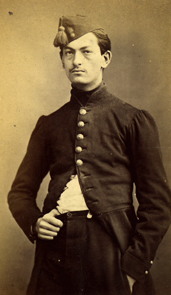
\includegraphics[width=\linewidth]{images/book3/b1-michel-levy.jpg}

{\scriptsize विद्यार्थी के रूप में मिशेल-लेवी, लगभग 1862। सार्वजनिक क्षेत्र।}
\end{minipage}
\end{history}

एक दूसरा, ज्ञात अतिरिक्त \omterm{def:b1:optical-mineralogy:retardation}{मंदन}, एक सहायक पट्टी द्वारा, जो ध्रुवकों के \ang{45} पर काट के ऊपर डाली जाती है, कणों से निकलती
दो तरंगों को दिया जा सकता है। सबसे आम पट्टी \omterm{def:b1:optical-mineralogy:interference-colour}{प्रथम कोटि} के लाल को दिखाने के लिए काटी जाती है, लगभग \qty{540}{nm} का \omterm{def:b1:optical-mineralogy:retardation}{मंदन}। यदि
कण की धीमी कंपन-दिशा पट्टी की धीमी दिशा के समांतर है, तो विलंब जुड़ते हैं और कण का रंग लगभग एक \omterm{def:b1:optical-mineralogy:interference-colour}{कोटि} ऊपर उठता है; यदि वह
तेज़ दिशा के समांतर है, तो वे घटते हैं और रंग गिरता है। \qty{100}{nm} का एक प्रथम-कोटि का धूसर कण एक अभिविन्यास में
द्वितीय-कोटि का नीला (\qty{640}{nm}) और दूसरे में प्रथम-कोटि का नारंगी (\qty{440}{nm}) बन जाता है; यह परीक्षण बताता है
कि कण की दो कंपन-दिशाओं में से कौन-सी धीमी है, एक ऐसा गुण जिसका उपयोग लंबे खनिजों को पहचानने में होता है।

\section{पतली काट में खनिजों की पहचान}

\begin{definition}[यमल, बहुसंश्लिष्ट यमलन]\label{def:b1:optical-mineralogy:twin}
एक \emph{यमल}\index{यमल (क्रिस्टल का)} एक ही \omterm{def:b1:rock-forming-minerals:mineral}{खनिज} के दो या अधिक क्रिस्टलों का अंतर्वृद्धि है जिनकी जालकें एक ऐसी समरूपता
से संबंधित हैं जो क्रिस्टल में स्वयं नहीं है, जैसे एक तल (यमल-तल) के आरपार परावर्तन। \emph{बहुसंश्लिष्ट यमलन}\index{बहुसंश्लिष्ट यमलन}
समांतर तलों पर बार-बार यमलन है, जो एक क्रिस्टल को पतले समांतर पटलों में बाँटता है जिनके अभिविन्यास बारी-बारी से होते हैं।
\end{definition}

\omterm{def:b1:field-lab-methods-1:microscope}{आड़े ध्रुवकों} के बीच एक बहुसंश्लिष्ट \omterm{def:b1:optical-mineralogy:twin}{यमल} के पटल बारी-बारी से विलोपित होते हैं: आधे काले होते हैं जब बाकी आधे चमकीले,
और क्रिस्टल धारीदार दिखता है। \omterm{def:b1:rock-forming-minerals:groups}{प्लैजियोक्लेज़} लगभग हमेशा ये धारियाँ दिखाता है, जो उसे स्फटिक और \omterm{def:b1:rock-forming-minerals:groups}{क्षारीय फ़ेल्सपार} से
तुरंत अलग करती हैं; उसकी दूसरी विशेषता, निम्न \omterm{def:b1:optical-mineralogy:relief}{उभार} और प्रथम-कोटि का धूसर से सफ़ेद रंग, वह उनके साथ साझा करता है। यमल-तल
के दोनों ओर मापे गए पटल-समुच्चयों के \omterm{def:b1:optical-mineralogy:extinction}{विलोपन कोण} \omterm{def:b1:rock-forming-minerals:groups}{प्लैजियोक्लेज़} के संघटन पर निर्भर करते हैं, और उन कोणों के चार्ट
उसका एनॉर्थाइट अंश देते हैं।

\begin{method}[पतली काट में एक खनिज की पहचान]\label{met:b1:optical-mineralogy:identify}
\begin{enumerate}
  \item \omterm{def:b1:field-lab-methods-1:microscope}{समतल-ध्रुवित प्रकाश} में: देखिए कि कण अपारदर्शी है या नहीं; उसका रंग और \omterm{def:b1:optical-mineralogy:pleochroism}{बहुवर्णता} (मंच घुमाइए); उसका \omterm{def:b1:optical-mineralogy:relief}{उभार}, और
        वह $1.54$ के किस ओर अपवर्तनांक रखता है (\omterm{def:b1:optical-mineralogy:relief}{बेक रेखा}); उसका आकार और विदलन, और दो विदलनों के बीच का कोण।
  \item \omterm{def:b1:field-lab-methods-1:microscope}{आड़े ध्रुवकों} के बीच: जाँचिए कि वह काला रहता है या नहीं (समदैशिक, या \omterm{def:b1:optical-mineralogy:optic-axis}{प्रकाशिक अक्ष} के लंबवत काट); एक ही \omterm{def:b1:rock-forming-minerals:mineral}{खनिज}
        के कणों में सबसे ऊँचा \omterm{def:b1:optical-mineralogy:interference-colour}{व्यतिकरण वर्ण} खोजिए, और काट की मोटाई के लिए \omterm{def:b1:optical-mineralogy:interference-colour}{माइकेल-लेवी चार्ट} पर \omterm{def:b1:optical-mineralogy:birefringence}{द्विअपवर्तन} पढ़िए।
  \item विदलन या दीर्घीकरण दिखाने वाले कणों पर \omterm{def:b1:optical-mineralogy:extinction}{विलोपन कोण} मापिए; यमलन (बहुसंश्लिष्ट धारियाँ, सरल \omterm{def:b1:optical-mineralogy:twin}{यमल}) खोजिए।
  \item खनिजों के प्रकाशिक गुणों की तालिका (\cref{tab:b1:optical-mineralogy:key}) और उन खनिजों से तुलना कीजिए जो चट्टान
        में हो सकते हैं (\cref{ch:b1:rock-forming-minerals})।
\end{enumerate}
\end{method}

\begin{table}[htbp]
\centering\footnotesize
\setlength{\tabcolsep}{3pt}
% ledger: hom:quartz-optics, hom:orthoclase-optics, hom:albite-optics, hom:anorthite-optics, hom:muscovite-optics, hom:biotite-optics, hom:hornblende-optics, hom:diopside-optics, hom:forsterite-optics, hom:fayalite-optics, hom:almandine-optics, hom:calcite-optics, hom:magnetite-optics
\begin{tabular}{@{}>{\raggedright\arraybackslash}p{2.0cm}>{\raggedright\arraybackslash}p{2.6cm}>{\raggedright\arraybackslash}p{2.3cm}>{\raggedright\arraybackslash}p{1.8cm}>{\raggedright\arraybackslash}p{3.0cm}>{\raggedright\arraybackslash}p{3.8cm}@{}}
\hline
\omterm{def:b1:rock-forming-minerals:mineral}{खनिज} & रंग (समतल-ध्रुवित) & अपवर्तनांक & \omterm{def:b1:optical-mineralogy:birefringence}{द्विअपवर्तन} & \qty{30}{\micro m} पर सबसे ऊँचा रंग & अन्य विशेषताएँ \\
\hline
स्फटिक & रंगहीन & 1.544--1.553 & 0.009 & प्रथम-कोटि का सफ़ेद & कोई विदलन नहीं; कोई \omterm{def:b1:optical-mineralogy:twin}{यमल} दिखाई नहीं देता; \omterm{def:b1:optical-mineralogy:optic-axis}{एकाक्षीय} \\
ऑर्थोक्लेज़ & रंगहीन, प्रायः धुँधला & 1.518--1.525 & 0.005 & प्रथम-कोटि का धूसर & ऋणात्मक \omterm{def:b1:optical-mineralogy:relief}{उभार}; सरल \omterm{def:b1:optical-mineralogy:twin}{यमल} \\
\omterm{def:b1:rock-forming-minerals:groups}{प्लैजियोक्लेज़} & रंगहीन & 1.526--1.590 & 0.008--0.013 & प्रथम-कोटि का सफ़ेद से हल्का पीला & \omterm{def:b1:optical-mineralogy:twin}{बहुसंश्लिष्ट यमलन} \\
मस्कोवाइट & रंगहीन & 1.552--1.618 & 0.035--0.042 & चमकीला द्वितीय- से तृतीय-कोटि & एक पूर्ण विदलन; सीधा विलोपन \\
बायोटाइट & भूरा, हरा & 1.565--1.696 & 0.04--0.07 & अपने ही रंग से ढका हुआ & प्रबल \omterm{def:b1:optical-mineralogy:pleochroism}{बहुवर्णता}; एक पूर्ण विदलन \\
हॉर्नब्लेंड & हरा, भूरा & 1.675--1.695 & 0.020 & द्वितीय-कोटि का नीला & \omterm{def:b1:optical-mineralogy:pleochroism}{बहुवर्णी}; \ang{56}/\ang{124} पर विदलन; विलोपन \ang{15}--\ang{19} \\
डायोप्साइड & रंगहीन & 1.664--1.694 & 0.030 & द्वितीय-कोटि का पीला & लगभग \ang{87}/\ang{93} पर विदलन; विलोपन लगभग \ang{38} \\
\omterm{def:b1:rock-forming-minerals:groups}{ओलिवीन} & रंगहीन (Mg) से हल्का पीला (Fe) & 1.635--1.879 & 0.035--0.052 & द्वितीय-कोटि के अंत से तृतीय-कोटि तक & ऊँचा \omterm{def:b1:optical-mineralogy:relief}{उभार}; अनियमित दरारें, कोई अच्छा विदलन नहीं \\
\omterm{def:b1:rock-forming-minerals:groups}{गार्नेट} & रंगहीन से हल्का गुलाबी & 1.830 (अल्माँडीन) & समदैशिक & काला & बहुत ऊँचा \omterm{def:b1:optical-mineralogy:relief}{उभार}; छह या आठ पार्श्वों वाली रूपरेखाएँ \\
कैल्साइट & रंगहीन & 1.486--1.658 & 0.172 & उच्च-कोटि का सफ़ेद & घूमने पर \omterm{def:b1:optical-mineralogy:relief}{उभार} बदलता है; समचतुर्भुजीय विदलन \\
मैग्नेटाइट & अपारदर्शी & --- & --- & --- & दोनों प्रकाशों में काला \\
\hline
\end{tabular}
\caption{\omterm{def:b1:field-lab-methods-1:thin-section}{पतली काट} में सामान्य शैल-निर्माता खनिजों के प्रकाशिक गुण।
PPL: \omterm{def:b1:field-lab-methods-1:microscope}{समतल-ध्रुवित प्रकाश}। सबसे ऊँचा रंग \omterm{def:b1:optical-mineralogy:interference-colour}{माइकेल-लेवी चार्ट} पर $\Delta = \qty{30000}{nm}\times\delta$ पर पढ़ा जाता है।}
\label{tab:b1:optical-mineralogy:key}
\end{table}

\begin{omfigure}
\setlength{\tabcolsep}{2pt}
\begin{tabular}{cc}
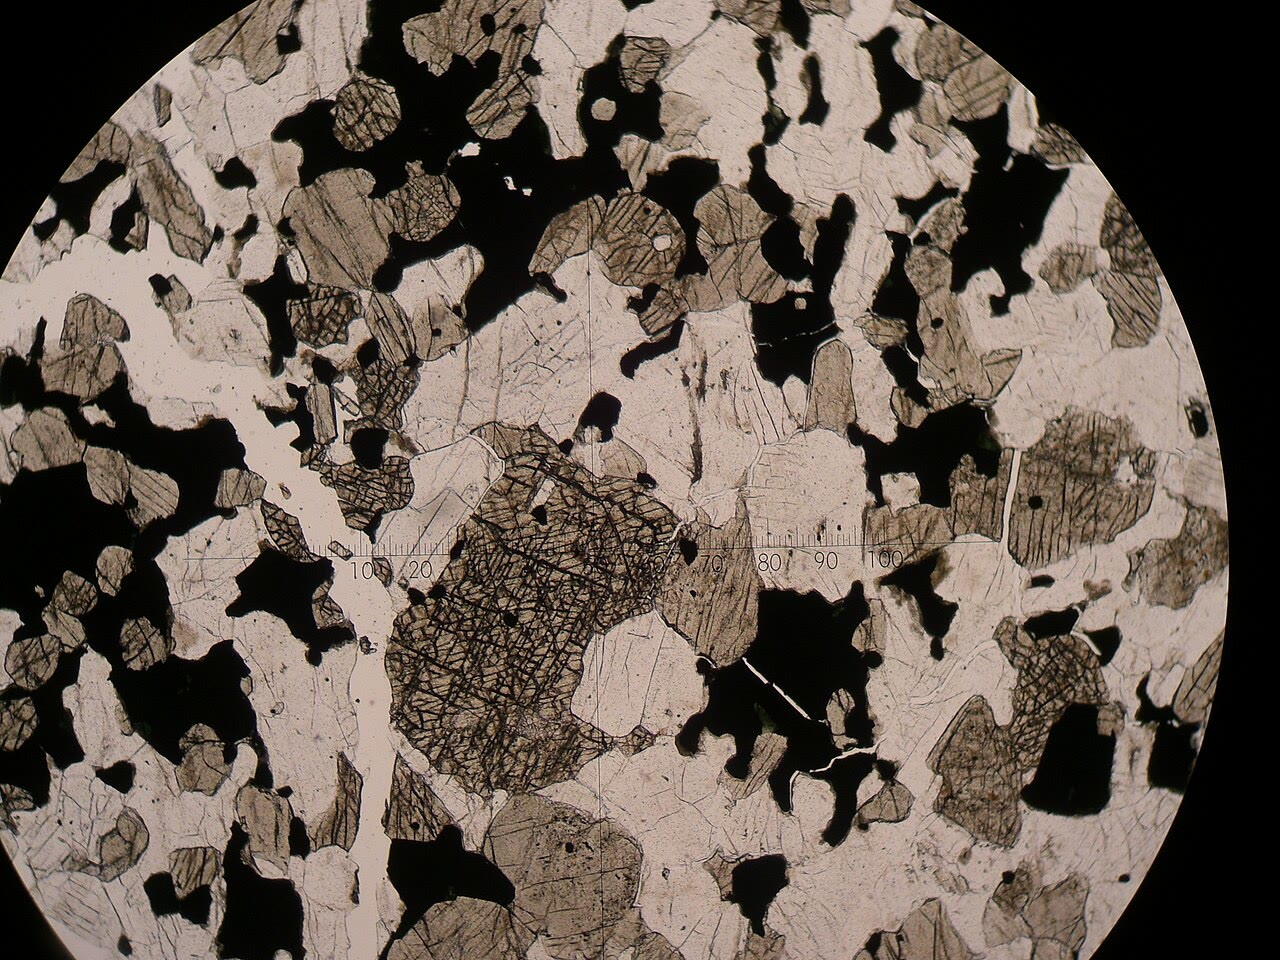
\includegraphics[width=0.485\linewidth]{images/book3/b1-gabbro-ppl.jpg} &
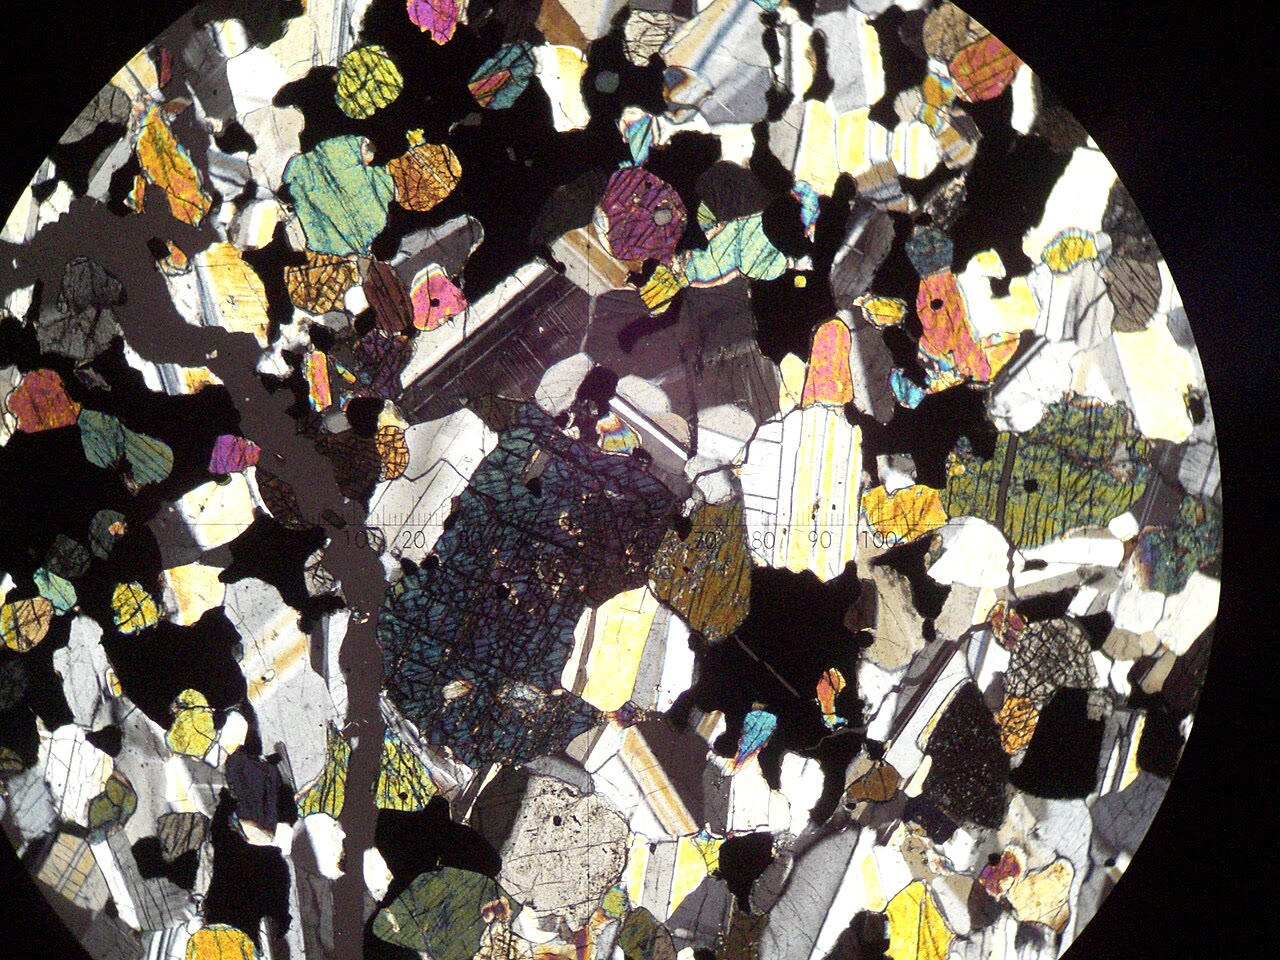
\includegraphics[width=0.485\linewidth]{images/book3/b1-gabbro-xpl.jpg} \\
{\small (क) \omterm{def:b1:field-lab-methods-1:microscope}{समतल-ध्रुवित प्रकाश}} & {\small (ख) \omterm{def:b1:field-lab-methods-1:microscope}{आड़े ध्रुवक}} \\
\end{tabular}
% ledger: commons:gabbro-ppl, commons:gabbro-xpl

\medskip
{\small एक गैब्रो की \omterm{def:b1:field-lab-methods-1:thin-section}{पतली काट} में वही क्षेत्र। \omterm{def:b1:field-lab-methods-1:microscope}{समतल-ध्रुवित प्रकाश} में (क) \omterm{def:b1:rock-forming-minerals:groups}{प्लैजियोक्लेज़} निम्न \omterm{def:b1:optical-mineralogy:relief}{उभार} वाला रंगहीन है, \omterm{def:b1:rock-forming-minerals:groups}{पाइरॉक्सीन}
और \omterm{def:b1:rock-forming-minerals:groups}{ओलिवीन} के कण उच्च \omterm{def:b1:optical-mineralogy:relief}{उभार} और घनी दरारों के साथ हल्के भूरे-धूसर हैं, और अपारदर्शी अयस्क काला है; पैमाना नेत्रिका में
एक माइक्रोमीटर है। \omterm{def:b1:field-lab-methods-1:microscope}{आड़े ध्रुवकों} के बीच (ख) \omterm{def:b1:rock-forming-minerals:groups}{प्लैजियोक्लेज़} की पट्टियाँ \omterm{def:b1:optical-mineralogy:twin}{बहुसंश्लिष्ट यमलन} से धारीदार हैं, \omterm{def:b1:rock-forming-minerals:groups}{पाइरॉक्सीन} और
\omterm{def:b1:rock-forming-minerals:groups}{ओलिवीन} के कण द्वितीय-कोटि के रंगों में चमकते हैं, और अयस्क काला रहता है। फ़ोटो Chmee2, CC BY-SA 3.0 (विकिमीडिया कॉमन्स)।}
\end{omfigure}

\begin{inthelab}[सूक्ष्मदर्शी पर एक सत्र]
\begin{minipage}[t]{0.55\linewidth}\vspace{0pt}
एक शैलविज्ञानी एक नई \omterm{def:b1:field-lab-methods-1:thin-section}{पतली काट} का वर्णन करते समय उसे पहले कम आवर्धन पर देखती है, ताकि बनावट और मुख्य \omterm{def:b1:rock-forming-minerals:mineral}{खनिज} दिखें,
फिर कण-दर-कण। हर \omterm{def:b1:rock-forming-minerals:mineral}{खनिज} के लिए वह इस विधि के प्रेक्षण दर्ज करती है, क्षेत्र में उसका अनुपात अनुमानित करती है, और नोट
करती है कि कण एक-दूसरे को कैसे छूते हैं: कौन पहले क्रिस्टलित हुआ, कौन छूटे स्थान भरता है, कौन दूसरों को प्रतिस्थापित
करता है। प्रकाशमिति के मापन अंशों में अंशांकित मंच और एक सहायक पट्टी के साथ होते हैं; संघटन, जब वह मायने रखता है,
बाद में उसी काट पर एक माइक्रोप्रोब से मापे जाते हैं। एक शिक्षण प्रयोगशाला उसी तरह काम करती है, हर विद्यार्थी के लिए एक
सूक्ष्मदर्शी और उसके बगल में ज्ञात खनिजों की संदर्भ-काटों की एक डिब्बी।
\end{minipage}\hfill
\begin{minipage}[t]{0.42\linewidth}\vspace{0pt}
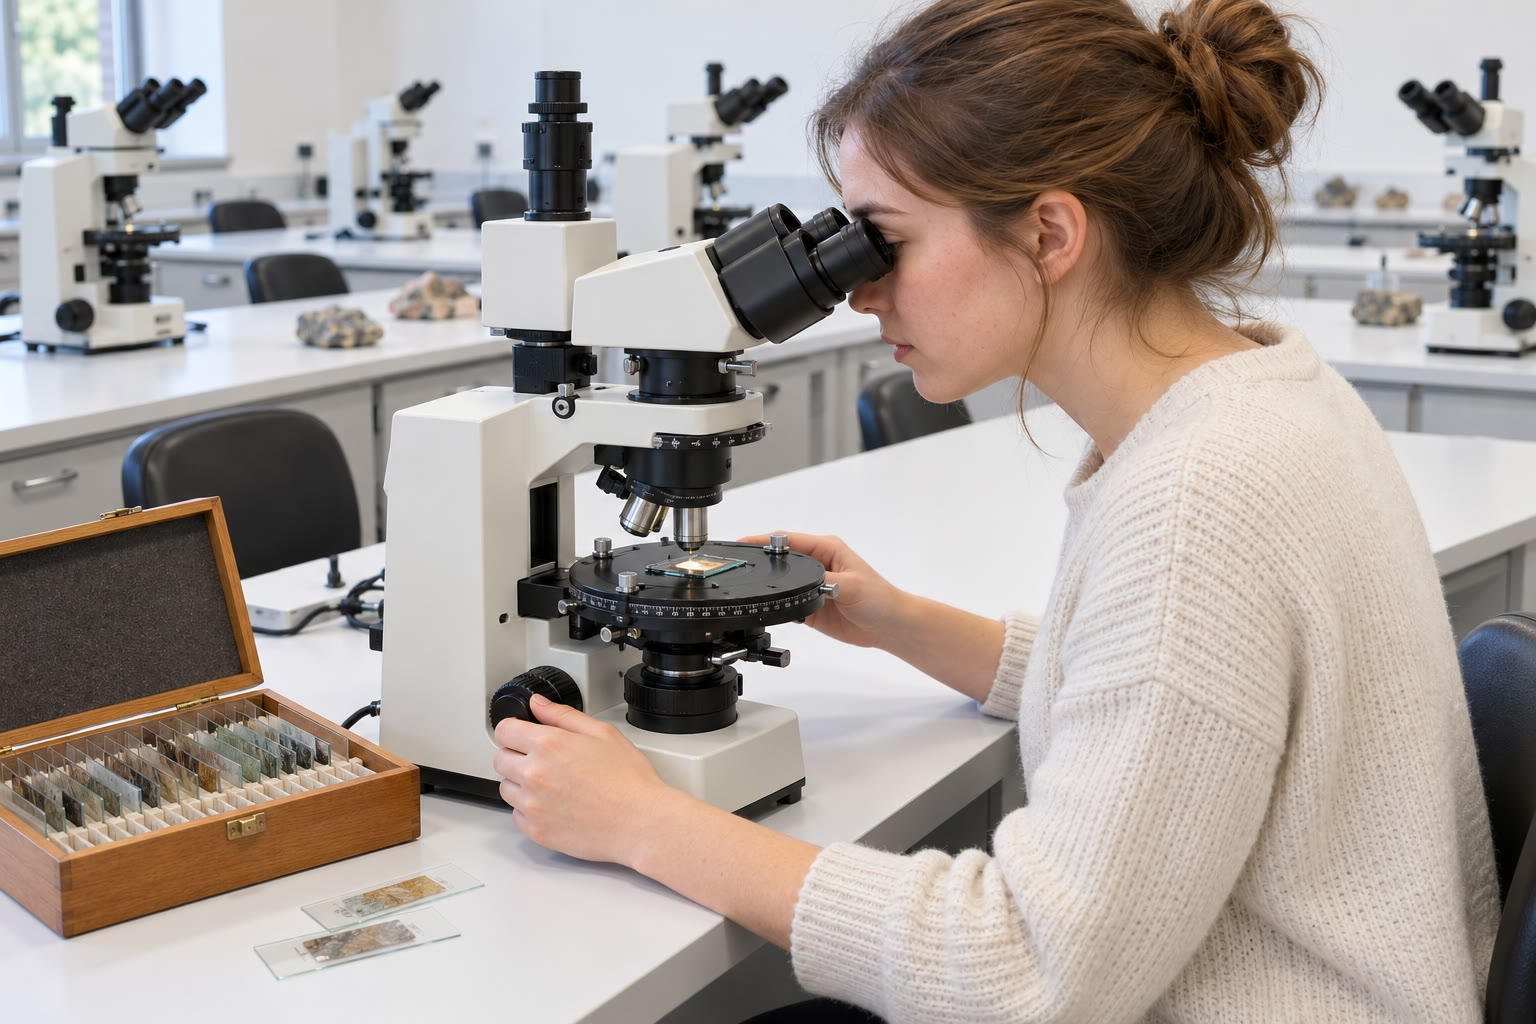
\includegraphics[width=\linewidth]{images/book3/ai/b1-microscope-student.jpg}

{\scriptsize शिक्षण प्रयोगशाला में \omterm{def:b1:field-lab-methods-1:microscope}{ध्रुवण सूक्ष्मदर्शी} पर एक विद्यार्थी (AI से बनी आकृति)।}
\end{minipage}
\end{inthelab}

\section{अभ्यास}

\begin{exercise}[$\star$]\label{exo:b1:optical-mineralogy:1}
\qty{30}{\micro m} मोटी काट में स्फटिक ($\delta = 0.009$) और कैल्साइट ($\delta = 0.172$) का सबसे बड़ा \omterm{def:b1:optical-mineralogy:retardation}{मंदन} परिकलित कीजिए।
\omterm{def:b1:optical-mineralogy:interference-colour}{माइकेल-लेवी चार्ट} से हर एक का रंग वर्णित कीजिए।
% ledger: hom:quartz-optics, hom:calcite-optics
\end{exercise}

\begin{exercise}[$\star$]\label{exo:b1:optical-mineralogy:2}
एक कण को \omterm{def:b1:field-lab-methods-1:microscope}{आड़े ध्रुवकों} के बीच मंच पर घुमाया जाता है। उसके अधिकतम का भाग $I/I_0$ \omterm{def:b1:optical-mineralogy:extinction}{विलोपन स्थिति} से $\theta = 0$, \ang{22.5},
\ang{45}, \ang{67.5} और \ang{90} पर परिकलित कीजिए।
\end{exercise}

\begin{exercise}[$\star$]\label{exo:b1:optical-mineralogy:3}
समझाइए कि \omterm{def:b1:rock-forming-minerals:groups}{गार्नेट} मंच की किसी भी स्थिति में \omterm{def:b1:field-lab-methods-1:microscope}{आड़े ध्रुवकों} के बीच काला क्यों रहता है, और स्फटिक का एक कण वही क्यों कर
सकता है। \omterm{def:b1:field-lab-methods-1:microscope}{समतल-ध्रुवित प्रकाश} में आप उन्हें कैसे अलग करेंगे?
\end{exercise}

\begin{exercise}[$\star$]\label{exo:b1:optical-mineralogy:4}
$1.54$ अपवर्तनांक के माध्यम में \omterm{def:b1:optical-mineralogy:relief}{उभार} के अनुसार क्रम दीजिए: ऑर्थोक्लेज़ ($n$ लगभग $1.52$), स्फटिक ($1.55$), फ़ॉर्स्टेराइट
($1.65$) और अल्माँडीन ($1.83$)। किसका \omterm{def:b1:optical-mineralogy:relief}{उभार} ऋणात्मक है? फ़ोकस ऊपर उठाने पर उसकी \omterm{def:b1:optical-mineralogy:relief}{बेक रेखा} किस दिशा में खिसकती है?
% ledger: hom:orthoclase-optics, hom:quartz-optics, hom:forsterite-optics, hom:almandine-optics
\end{exercise}

\begin{exercise}[$\star\star$]\label{exo:b1:optical-mineralogy:5}
\qty{30}{\micro m} काट में, दो विदलनों वाले, \ang{56} और \ang{124} पर, एक हरे \omterm{def:b1:optical-mineralogy:pleochroism}{बहुवर्णी} \omterm{def:b1:rock-forming-minerals:mineral}{खनिज} के कण अधिक-से-अधिक द्वितीय-कोटि का
नीला दिखाते हैं, जिसे चार्ट पर $\Delta = \qty{650}{nm}$ पढ़ा जाता है। उसका \omterm{def:b1:optical-mineralogy:birefringence}{द्विअपवर्तन} परिकलित कीजिए और तालिका से \omterm{def:b1:rock-forming-minerals:mineral}{खनिज} का नाम
बताइए।
\end{exercise}

\begin{exercise}[$\star\star$]\label{exo:b1:optical-mineralogy:6}
\cref{prop:b1:optical-mineralogy:relief} का उपयोग करके, $n_m = 1.54$ और $i = \ang{30}$ के साथ, एक स्फटिक कण ($n = 1.553$)
और एक फ़ॉर्स्टेराइट कण ($n = 1.651$) की कोर पर विचलन, अंशों में, और दोनों का अनुपात परिकलित कीजिए। दूसरे की स्नेल के
नियम से ठीक-ठीक जाँच कीजिए।
\end{exercise}

\begin{exercise}[$\star\star$]\label{exo:b1:optical-mineralogy:7}
एक प्रथम-कोटि के लाल पट्टी का $\Delta = \qty{540}{nm}$ है। $\Delta = \qty{270}{nm}$ वाला एक स्फटिक कण पट्टी डालकर \ang{45} पर
रखा जाता है। दो संभावित कुल \omterm{def:b1:optical-mineralogy:retardation}{मंदन} क्या हैं, और चार्ट पर वे कौन-से रंग देते हैं? कौन-सा अभिविन्यास दोनों धीमी दिशाओं को
समांतर रखता है?
\end{exercise}

\begin{exercise}[$\star\star$]\label{exo:b1:optical-mineralogy:8}
अपनी पतली होती कोर पर, $\delta = 0.052$ वाला एक फ़ायलाइट कण \qty{30}{\micro m} से शून्य तक पतला होता है। कोर और कण के पूर्ण-मोटाई
भाग के बीच की झालरों के रूप में, 542, 1074 और \qty{1605}{nm} पर कोटियों को समाप्त करने वाली कितनी लाल-बैंगनी आभाएँ
रंगीन झालरों के रूप में दिखती हैं?
% ledger: hom:fayalite-optics
\end{exercise}

\begin{exercise}[$\star\star$]\label{exo:b1:optical-mineralogy:9}
एक अच्छे विदलन वाले कई लंबे कणों पर एक शैलविज्ञानी विदलन-रेखा और धीमी कंपन-दिशा के बीच \ang{0}, \ang{21}, \ang{36} और
\ang{37} के \omterm{def:b1:optical-mineralogy:extinction}{विलोपन कोण} मापता है। मान क्यों भिन्न हैं? क्या \omterm{def:b1:rock-forming-minerals:mineral}{खनिज} अधिक संभवतः डायोप्साइड है या हॉर्नब्लेंड?
% ledger: hom:diopside-optics, hom:hornblende-optics
\end{exercise}

\begin{exercise}[$\star\star\star$]\label{exo:b1:optical-mineralogy:10}
\cref{thm:b1:optical-mineralogy:intensity} की उपपत्ति को विश्लेषक को ध्रुवक के समांतर रखकर दोहराइए, और दिखाइए कि
$I_\parallel = I_0\bigl(1 - \sin^2 2\theta\sin^2(\pi\Delta/\lambda)\bigr)$। $\Delta = \qty{550}{nm}$ वाला एक कण समांतर ध्रुवकों
के बीच \ang{45} पर कौन-सा रंग दिखाता है?
\end{exercise}

\begin{exercise}[$\star\star\star$]\label{exo:b1:optical-mineralogy:11}
$\Delta = \qty{5000}{nm}$ वाले एक कैल्साइट कण के लिए, गुणक $\sin^2(\pi\Delta/\lambda)$ जब भी $\Delta/\lambda$ एक पूर्ण
संख्या हो, शून्य होता है। (क) \num{400} और \qty{700}{nm} के बीच यह कितनी बार शून्य होता है? (ख) दिखाइए कि
$\lambda = \qty{550}{nm}$ के निकट दो क्रमागत शून्य लगभग $\lambda^2/\Delta$ दूर हैं, और उसे परिकलित कीजिए। (ग) समझाइए कि
कण लगभग सफ़ेद क्यों दिखता है।
\end{exercise}

\begin{exercise}[$\star\star\star$]\label{exo:b1:optical-mineralogy:12}
दिखाइए कि मंच के एक पूरे चक्कर पर औसत लेने पर, \omterm{def:b1:field-lab-methods-1:microscope}{आड़े ध्रुवकों} के बीच एक कण $\frac12 I_0\sin^2(\pi\Delta/\lambda)$ गुज़रने देता है।
एक शैलविज्ञानी \qty{30}{\micro m} मानकर हर \omterm{def:b1:rock-forming-minerals:mineral}{खनिज} के सबसे ऊँचे रंग से \omterm{def:b1:optical-mineralogy:birefringence}{द्विअपवर्तन} अनुमानित करती है, जबकि काट वास्तव में
\qty{25}{\micro m} मोटी है। उसके सभी मान किस गुणक से गलत हैं, और किस दिशा में?
\end{exercise}

\section{समस्या: एक अज्ञात पतली काट के खनिज पहचानना}

\begin{problem}[{सप्ताहांत समस्या --- उभार, बहुवर्णता और व्यतिकरण वर्णों का प्रेक्षण, स्फटिक के साथ काट की मोटाई मापना,
और उसके खनिजों के नाम रखना}]
\label{pb:b1:optical-mineralogy:1}
% values: calc/ch08.py; optical data: ledger hom:*-optics
% ledger: hom:quartz-optics, hom:diopside-optics, hom:forsterite-optics, hom:albite-optics, hom:anorthite-optics, hom:hornblende-optics, hom:biotite-optics
एक अज्ञात आग्नेय चट्टान की \omterm{def:b1:field-lab-methods-1:thin-section}{पतली काट}, $1.540$ अपवर्तनांक के एक रेज़िन में आरोपित, \qty{30}{\micro m} मोटी बताई जाती है।
उसमें पाँच \omterm{def:b1:rock-forming-minerals:mineral}{खनिज} हैं, जिन्हें A से E तक नामित किया गया है। अध्याय की प्रकाशिक गुणों की तालिका, \omterm{def:b1:optical-mineralogy:interference-colour}{माइकेल-लेवी चार्ट}, और
ये मान उपयोग कीजिए: स्फटिक $n_\omega = 1.544$, $n_\varepsilon = 1.553$; डायोप्साइड $n_\alpha = 1.664$, $n_\beta = 1.672$,
$n_\gamma = 1.694$।

\medskip
\noindent\textbf{भाग I --- समतल-ध्रुवित प्रकाश।}
\begin{enumerate}
  \item \omterm{def:b1:rock-forming-minerals:mineral}{खनिज} A रंगहीन है, जिसकी कण-सीमाएँ मुश्किल से दिखती हैं। \omterm{def:b1:rock-forming-minerals:mineral}{खनिज} B रंगहीन है, जिसकी प्रबल गहरी किनारियाँ हैं और दो विदलन
        लगभग \ang{87} पर मिलते हैं। किसका \omterm{def:b1:optical-mineralogy:relief}{उभार} अधिक है?
  \item A को स्फटिक, और B को डायोप्साइड मानकर, हर एक के मुख्य अपवर्तनांकों के माध्य से $|n - n_m|$ परिकलित कीजिए।
  \item \cref{prop:b1:optical-mineralogy:relief} का उपयोग करके, सीमा के समान झुकाव के लिए उनकी कोरों पर विचलनों का अनुपात
        परिकलित कीजिए।
  \item फ़ोकस ऊपर उठाने पर B की \omterm{def:b1:optical-mineralogy:relief}{बेक रेखा} कण के भीतर खिसकती है। यह क्या दिखाता है?
  \item \omterm{def:b1:rock-forming-minerals:mineral}{खनिज} C मंच घूमने पर हल्के पीले से गहरे भूरे में बदलता है, सबसे गहरा तब जब उसका एकल विदलन ध्रुवक के अनुदिश हो।
        गुण और \omterm{def:b1:rock-forming-minerals:mineral}{खनिज} का नाम बताइए।
  \item \omterm{def:b1:rock-forming-minerals:mineral}{खनिज} D रंगहीन है, निम्न \omterm{def:b1:optical-mineralogy:relief}{उभार} वाला, लंबी पट्टियों में; E हरे से पीले तक और \omterm{def:b1:optical-mineralogy:pleochroism}{बहुवर्णी} है, \ang{124} पर दो विदलनों के साथ।
        कोण E के बारे में क्या सुझाता है?
\end{enumerate}

\medskip
\noindent\textbf{भाग II --- काट की मोटाई।}
\begin{enumerate}[resume]
  \item ठीक \qty{30}{\micro m} की काट में स्फटिक का सबसे बड़ा \omterm{def:b1:optical-mineralogy:retardation}{मंदन} क्या है? उसका रंग क्या है?
  \item A के कई कणों में सबसे बड़ा \omterm{def:b1:optical-mineralogy:retardation}{मंदन} क्यों खोजना होगा, किसी एक पर मापने के बजाय?
  \item A के कणों द्वारा दिखाया गया सबसे ऊँचा रंग प्रथम-कोटि का हल्का पीला है; एक स्फटिक-पच्चर तुलनित्र उसका \omterm{def:b1:optical-mineralogy:retardation}{मंदन} \qty{342}{nm} देता
        है। काट की \omterm{def:b1:cross-sections:thickness}{वास्तविक मोटाई} परिकलित कीजिए।
  \item काट कितने प्रतिशत उससे मोटी है जितनी उसे होना चाहिए?
  \item $\lambda = \qty{550}{nm}$ पर और विलोपन से \ang{45} पर, इस स्फटिक कण के लिए $I/I_0$ परिकलित कीजिए, और वही कण
        \qty{30}{\micro m} की काट में।
  \item D के \omterm{def:b1:optical-mineralogy:retardation}{मंदन} का परास परिकलित कीजिए, जिसे \omterm{def:b1:rock-forming-minerals:groups}{प्लैजियोक्लेज़} मानकर ($\delta = 0.008$ से $0.013$), इस काट में; और बताइए कि
        क्या उसके रंग \omterm{def:b1:optical-mineralogy:interference-colour}{प्रथम कोटि} में रहते हैं।
\end{enumerate}

\medskip
\noindent\textbf{भाग III --- B का द्विअपवर्तन।}
\begin{enumerate}[resume]
  \item B का सबसे ऊँचा रंग एक नीला है जिसे $\Delta = \qty{1140}{nm}$ पढ़ा जाता है। वह किस \omterm{def:b1:optical-mineralogy:interference-colour}{कोटि} में है?
  \item प्रश्न 9 में मिली मोटाई से B का \omterm{def:b1:optical-mineralogy:birefringence}{द्विअपवर्तन} परिकलित कीजिए।
  \item \qty{30}{\micro m} मानने पर कौन-सा \omterm{def:b1:optical-mineralogy:birefringence}{द्विअपवर्तन} मिलता? कौन-सा उच्च \omterm{def:b1:optical-mineralogy:relief}{उभार} वाला रंगहीन \omterm{def:b1:rock-forming-minerals:mineral}{खनिज} इसका सुझाव देता, और वह स्फटिक
        वाली चट्टान में क्यों असंगत है (विचार कीजिए \ce{Mg2SiO4 + SiO2 -> 2 MgSiO3})?
  \item प्रश्न 14 के परिणाम की तालिका से तुलना कीजिए, B के \omterm{def:b1:optical-mineralogy:relief}{उभार} और विदलनों के साथ, और निष्कर्ष निकालिए।
  \item एक सही \qty{30}{\micro m} काट में B अधिक-से-अधिक किस रंग का दिखेगा?
  \item काट को \qty{30}{\micro m} तक घिसा जाता है। उसे कितना पतला करना होगा, और तब स्फटिक का सबसे ऊँचा रंग क्या है?
\end{enumerate}

\medskip
\medskip
\noindent\textbf{भाग IV --- विलोपन और यमलन।}
\begin{enumerate}[resume]
  \item D की पट्टियाँ समांतर धारियों में बँटी हैं जो बारी-बारी से विलोपित होती हैं। विशेषता और \omterm{def:b1:rock-forming-minerals:mineral}{खनिज} का नाम बताइए।
  \item एक पट्टी की धारियाँ यमल-तल के दोनों ओर \ang{27} और \ang{28} पर विलोपित होती हैं। ऐसे कोण, कई पट्टियों पर मापे गए,
        प्रकाशित चार्टों से तुलना करने पर क्या देते हैं?
  \item E की विदलनों और उसकी धीमी दिशा के बीच सबसे ऊँचा \omterm{def:b1:optical-mineralogy:extinction}{विलोपन कोण} \ang{17} है। E का नाम बताइए।
  \item इस काट में E का सबसे बड़ा \omterm{def:b1:optical-mineralogy:retardation}{मंदन} और वह रंग परिकलित कीजिए जो वह दिखाता है।
  \item B का एक कण एक पूरे चक्कर में काला रहता है। समझाइए कि वह B के चमकीले कणों का वही \omterm{def:b1:rock-forming-minerals:mineral}{खनिज} कैसे हो सकता है।
  \item \omterm{def:b1:rock-forming-minerals:mineral}{खनिज} A से E तक सूचीबद्ध कीजिए, और बताइए कि वे किस प्रकार की चट्टान बनाते हैं।
  \item काट की \omterm{def:b1:cross-sections:thickness}{वास्तविक मोटाई}, माइक्रोमीटर में, क्या है?
\end{enumerate}
\end{problem}
